\documentclass[unicode,11pt,a4paper,oneside,numbers=endperiod,openany]{scrartcl}

\usepackage{ifthen}
\usepackage[utf8]{inputenc}
\usepackage{graphics}
\usepackage{graphicx}
\usepackage{hyperref}
%%%%%%%%%%%%%%%%%%%%% Added Packages: %%%%%%%%%%%%%%%%%%%%%%%%%%%%%%%%%%
\usepackage{amsmath}
\usepackage{float}

\usepackage[dvipsnames]{xcolor}
\usepackage{fancyvrb}

\usepackage{subcaption}
\usepackage{ifthen}
\usepackage{listings}



% redefine \VerbatimInput
\RecustomVerbatimCommand{\VerbatimInput}{VerbatimInput}%
{fontsize=\footnotesize,
 %
 frame=lines,  % top and bottom rule only
 framesep=2em, % separation between frame and text
 rulecolor=\color{Gray},
 %
%  label=\fbox{\color{Black}slurm-euler\_phase\_1.txt},
%  labelposition=topline,
 %
 commandchars=\|\(\), % escape character and argument delimiters for
                      % commands within the verbatim
 commentchar=*        % comment character
}

% \newcommand{\myInputFile}{slurm-euler_phase_1.txt} % Set the default input file
% \newboolean{isPhaseOne}
% \setboolean{isPhaseOne}{true} % Set to false for phase 2

% % Redefine \VerbatimInput
% \RecustomVerbatimCommand{\VerbatimInput}{VerbatimInput}%
% {
%     fontsize=\footnotesize,
%     frame=lines,  % top and bottom rule only
%     framesep=2em, % separation between frame and text
%     rulecolor=\color{Gray},
%     label=\fbox{\ifthenelse{\boolean{isPhaseOne}}{\color{Black}slurm-euler\_phase\_1.txt}{\color{Black}slurm-euler\_phase\_2.txt}},
%     labelposition=topline,
%     commandchars=\|\(\), % escape character and argument delimiters for
%                           % commands within the verbatim
%     commentchar=*        % comment character
% }
%%%%%%%%%%%%%%%%%%%%%%%%%%%%%%%%%%%%%%%%%%%%%%%%%%%%%%%%%%%%%%%%%%%%%%%

\pagestyle{plain}
\voffset -5mm
\oddsidemargin  0mm
\evensidemargin -11mm
\marginparwidth 2cm
\marginparsep 0pt
\topmargin 0mm
\headheight 0pt
\headsep 0pt
\topskip 0pt        
\textheight 255mm
\textwidth 165mm

\newcommand{\duedate} {}
\newcommand{\setduedate}[1]{%
\renewcommand\duedate {Due date:~ #1}}
\newcommand\isassignment {false}
\newcommand{\setassignment}{\renewcommand\isassignment {true}}
\newcommand{\ifassignment}[1]{\ifthenelse{\boolean{\isassignment}}{#1}{}}
\newcommand{\ifnotassignment}[1]{\ifthenelse{\boolean{\isassignment}}{}{#1}}

\newcommand{\assignmentpolicy}{
\begin{table}[h]
\begin{center}
\scalebox{0.8} {%
\begin{tabular}{|p{0.02cm}p{16cm}|}
\hline
&\\
\multicolumn{2}{|c|}{\Large\textbf{HPC Lab for CSE 2024 ---  Submission Instructions}}\\
\multicolumn{2}{|c|}{\large\textbf{(Please, notice that following instructions are mandatory: }}\\
\multicolumn{2}{|c|}{\large\textbf{submissions that don't comply with, won't be considered)}}\\
&\\
\textbullet & Assignments must be submitted to \href{https://moodle-app2.let.ethz.ch/course/view.php?id=22516}{Moodle} (i.e. in electronic format).\\
\textbullet & Provide both executable package and sources (e.g. C/C++ files, Matlab). 
If you are using libraries, please add them in the file. Sources must be organized in directories called:\\
\multicolumn{2}{|c|}{\textit{Project\_number\_lastname\_firstname}}\\
& and  the  file must be called:\\
\multicolumn{2}{|c|}{\textit{project\_number\_lastname\_firstname.zip}}\\
\multicolumn{2}{|c|}{\textit{project\_number\_lastname\_firstname.pdf}}\\
\textbullet &  The TAs will grade your project by reviewing your project write-up, and looking at the implementation 
                 you attempted, and benchmarking your code's performance.\\

\textbullet & You are allowed to discuss all questions with anyone you like; however: (i) your submission must list anyone you discussed problems with and (ii) you must write up your submission independently.\\
\hline
\end{tabular}
}
\end{center}
\end{table}
}
\newcommand{\punkte}[1]{\hspace{1ex}\emph{\mdseries\hfill(#1~\ifcase#1{Points}\or{Points}\else{Points}\fi)}}


\newcommand\serieheader[6]{
\thispagestyle{empty}%
\begin{flushleft}

\includegraphics[width=0.4\textwidth]{Images/ETHlogo_13}
\end{flushleft}
  \noindent%
  {\large\ignorespaces{\textbf{#1}}\hspace{\fill}\ignorespaces{ \textbf{#2}}}\\ \\%
  {\large\ignorespaces #3 \hspace{\fill}\ignorespaces #4}\\
  \noindent%
  \bigskip
  \hrule\par\bigskip\noindent%
  \bigskip {\ignorespaces {\Large{\textbf{#5}}}
  \hspace{\fill}\ignorespaces \large \ifthenelse{\boolean{\isassignment}}{\duedate}{#6}}
  \hrule\par\bigskip\noindent%  \linebreak
 }

\makeatletter
\def\enumerateMod{\ifnum \@enumdepth >3 \@toodeep\else
      \advance\@enumdepth \@ne
      \edef\@enumctr{enum\romannumeral\the\@enumdepth}\list
      {\csname label\@enumctr\endcsname}{\usecounter
        {\@enumctr}%%%? the following differs from "enumerate"
	\topsep0pt%
	\partopsep0pt%
	\itemsep0pt%
	\def\makelabel##1{\hss\llap{##1}}}\fi}
\let\endenumerateMod =\endlist
\makeatother




\usepackage{textcomp}






\begin{document}


\setassignment
\setduedate{25 March 2024, 23:59}

\serieheader{High-Performance Computing Lab for CSE}{2024}
            {Student: Yannick Ramic}
            {Discussed with: Carla Lopez}{Solution for Project 2}{}
\newline

\assignmentpolicy

\section{Computing $\pi$ with \texttt{OpenMP} [20 points]}
The very first exercise task, comprises of two subtasks, where the goal of this omp introductory exercise is to 
implement two versions of parallelized code. The underlying serial implementation is already given and provides 
the template on how to compute $\pi$ numerically, by approximating the integral with the midpoint rule, as explained 
in the exercise sheet. To speed up this task we should implement 2 different parallelized versions, one with the 
\textit{critical} directive and the other one with the \textit{reduction} clause. Besides the lecture notes the 
information to solve this task was taken from the introductory book by Hager and Wellein \cite{HPC}.
\newline \indent
As described in \cite{HPC}, OpenMP provides a more elegant way, compared to an implementation with a critical region, 
in order to update a variable. Thus, I will start with explaining the advantage of using the \textit{Reduction} clause.
The \textit{Reduction} clause expects a definition of the used operator, which is in our case the $+$ operator because 
we accumulate values at each iteration, by simply summing over them. Besides the operator we have to define our target 
value, which is in this case \textit{sum}. As a result, the specified variable will be privatized and initialized with 
a sensible initial value. In the end, obviously we need to synchronize each thread again. Thus, in the end all partial results 
in this case will be accumulated and stored in the variable sum. \cite{HPC}
\newline \indent
Another possibility, also described in \cite{HPC}, is to define critical regions, in order to achieve a fast parallelized 
version of a serial code implementation. Critical regions can become necessary, in order to avoid concurrent overwriting and 
sharing a variable. This problem is called race condition and can be avoided by allowing only one thread executing code in this 
defined code part. The order in which threads access this region of code is undefined but also here are possibilities if 
necessary. At this point it's important to mention that a wrong use of the \textit{critical} directive can lead to another 
problem called deadlocks, where one or more threads become inactivate and wait for resources that become never available. 
This problem typically occurs when two or more critical regions are badly arranged. For instance, when a thread encounters 
another critical directive inside a critical region, it will be blocked forever. In order to avoid this, OpenMP also provides 
the solution of naming the critical region, which offers the opportunity to distinguish each region. \cite{HPC}
\begin{figure}[H]
  \centering
  {\fontsize{8}{10}\selectfont
  \VerbatimInput{Images_Output/critical_reduction.txt}}
  \caption{Critical and Reduction Based Parallelization Version}
  \label{fig:critical_reduction}
\end{figure}
\indent
Before presenting the strong and weak scaling analysis, the underlying code for both versions can be found in 
\ref{fig:critical_reduction}. As mentioned in the last task it's necessary to benchmark the performance of each parallelized 
version. Thus, Wermelinger \cite{scaling} describes weak scaling by asking the question: How well does the prallel fraction scale 
among p processors? According to \cite{scaling} weak scaling can be summarized with a fixed execution time and identifying, 
how much longer it takes for the problem without parallelism. Whereas strong scaling has a fixed problem size and answers the question, 
how much does parallelism reduce the execution time of a problem.
\begin{align*}
  S_{p} = \frac{w/t_p}{w/t_1} = \frac{t_1}{t_p}
\end{align*}
\indent
The equation presented above describes the calculation of the speedup considering the strong scaling analysis, where w is the associated 
work or in other words the problem size, $t_1$ the time needed to complete the serial task and $t_p$ the time necessary to complete the 
described work in a parallelized fashion. On the other hand, in the equation beneath, $E_w$ represents the efficiency by using parallelism 
and this is considered as the weak scaling analysis. The big difference is that for the weak scaling we actually need to compute a solution 
for the serial implementation for different problem sizes. This is not necessary for the strong scaling, since the problem size is fixed. 
Thus, week scaling requires to compare the time it takes between the serial implementation for a specific problem size with the parallelized 
solution for the same problem size. From a starting value it is necessary to scale the problem up in size and with used threads. How this 
was done exactly for the underlying problem will become clear, by inspecting the provided output files. \cite{HPC}, \cite{scaling}
\begin{align*}
  S_{p} &= \frac{p \cdot w/t_p}{w/t_1} = p \cdot \frac{t_1}{t_p}\\
  E_{w} &= \frac{S_p}{p} = \frac{t_1}{t_p}
\end{align*}
\indent
The results from the provided codes, can be seen for both scaling analysis in the figures \ref{fig:strong_scaling} and \ref{fig:weak_scaling}.
It becomes evident from figure \ref{fig:strong_scaling} that initially the speedup is close to the ideal line, but at some point the results 
become worse. There are several reasons for this phenomena. First, the problem size is still too small to analyse the problem properaly. Even, 
with a size of 10 million iterations the code only takes 0.18 seconds to run. Since creating the team of threads and the two operations fork and 
join also require some time, this will result in the fact that splitting up the task between different threads takes more time than just 
solving the problem in a sequential and naive way. This is true for both, the critical and the reduction version. Also due to the waiting 
of threads in the critical case, ideally the reduction clause should lead to better and faster results. Eventhough I took 100 experiments and 
averaged the time, it becomes evident from both figures \ref{fig:strong_scaling} and \ref{fig:weak_scaling}, that the results for the 
reduction based solution zigzags around and this effect can't be seen. Mentionable is that at the last measurement in figure \ref{fig:strong_scaling} 
for the reduction based solution there is a spike up and a massive increasement in speedup.
% \newpage
\begin{figure}[H]
    \centering
    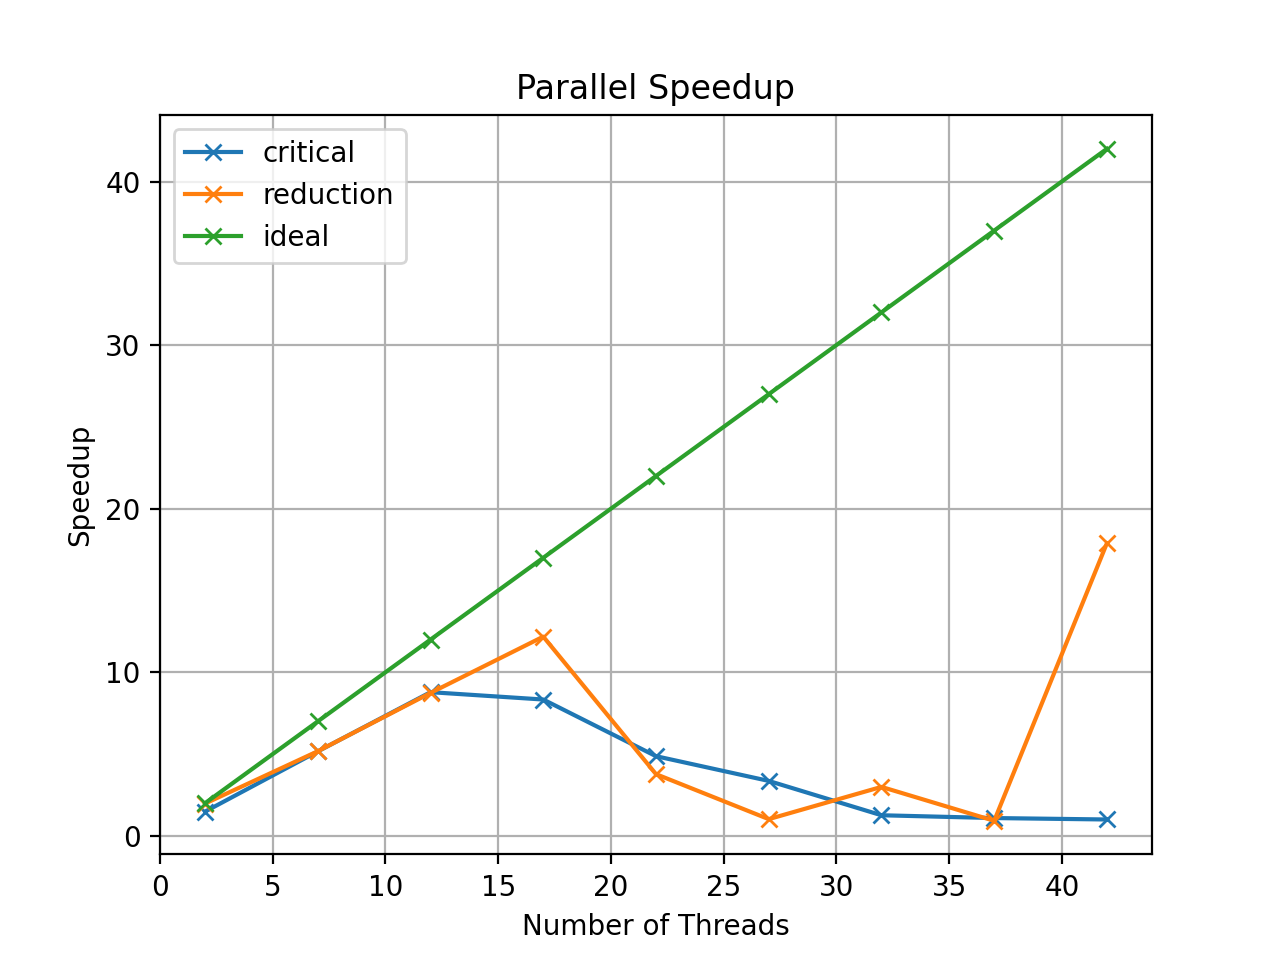
\includegraphics[width=\textwidth]{Images_Output/parallel_speedup.png}
    \caption{Strong Scaling Analysis: Parallel Speedup}
    \label{fig:strong_scaling}
  \end{figure}
\begin{figure}[H]
    \centering
    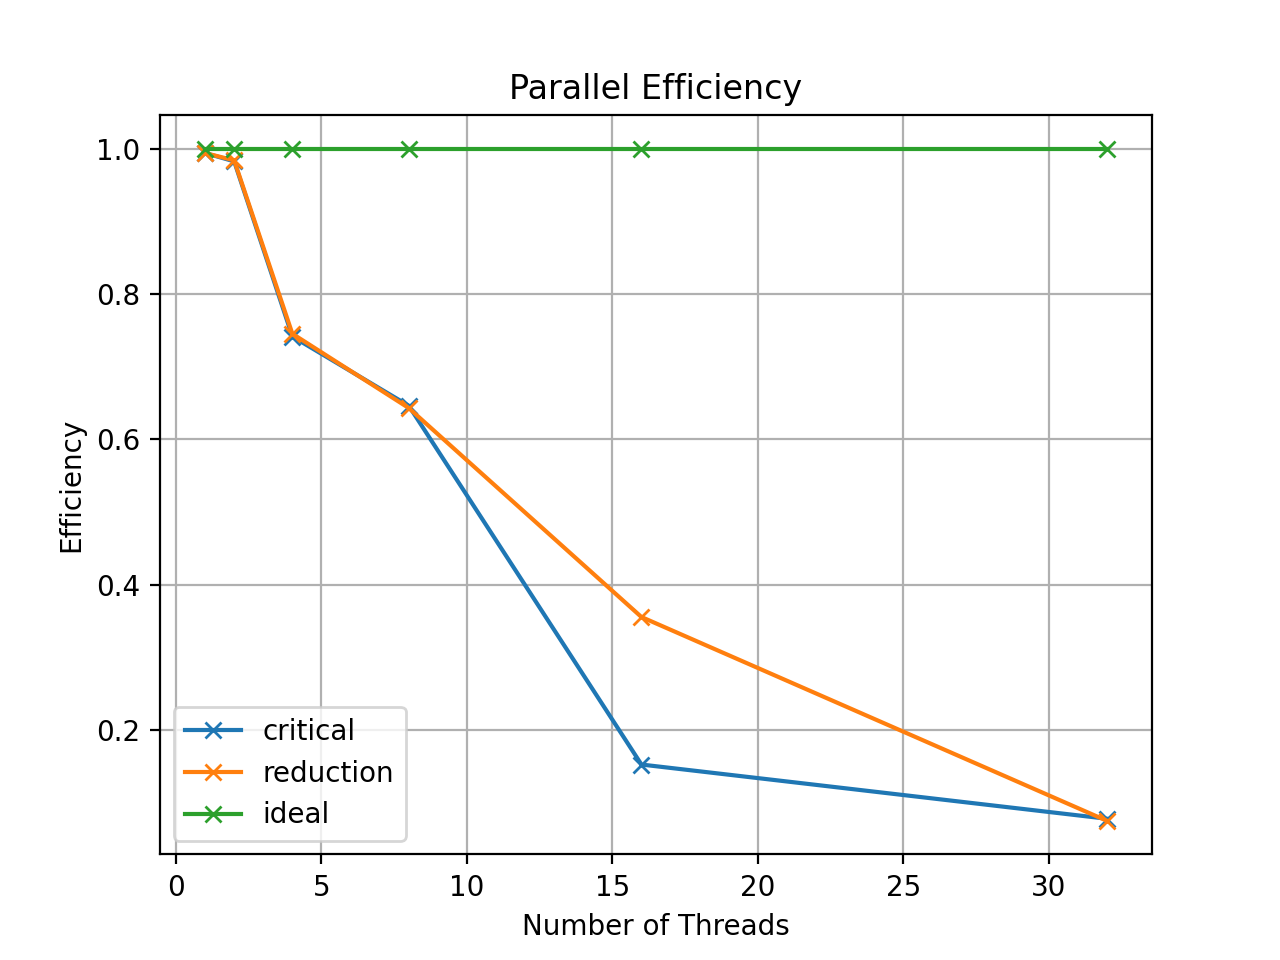
\includegraphics[width=\textwidth]{Images_Output/parallel_efficiency.png}
    \caption{Weak Scaling Analysis: Parallel Efficiency}
    \label{fig:weak_scaling}
  \end{figure}

\section{The Mandelbrot set  using \texttt{OpenMP} [20 points]}
\indent
The goal of this task is to visualize the Mandelbrot set and achieve this in a parallelized fashion. The visualized result can be seen 
in figure \ref{fig:mandel}. It becomes evident that on the left half plane there is a white line, which shouldn't be there compared to 
the sequential solution. The reason for this phenomena is simply double precision floating point errors that result in a few wrong results, 
where the underlying pixel doesn't have the value of 0, but some really small number instead.
\newline \indent
Compared to Chapter 1 the results seem more "stable". In figure \ref{fig:s_mandel} we see a linear instead of a zigzagging 
behaviour, by increasing the number of threads for a fixed problem size. For the same reasons as explained already in Chapter 1, that 
the process to fork the master thread into a team of threads and in the end joining them back together into the master thread again 
requires some time itself and is not a "perfect" operation without any time loss. Hence, there will be always a gap between the ideal 
and the actual behaviour of the parallelization speedup. Further results such as the underyling output file or a snapshot of it can be found 
in the Appendix, more precisly figure \ref{fig:output_mandel}.
\newline \indent
It is worth noting that for updating the variable nTotalIterationsCount, racing condition needs to be avoided. Instead of critical pragma 
here the pragma atomic was chosen, which share a lot of similarities. To run the code with multiple threads the pragma omp for was chosen 
without a collapse clause to make the code even faster. The colapse pragma would allow us to run both for loops in parallel and not only 
the first one. The main difficulty of this task was to think about classifying variables as private and shared. Also, the two values 
cx and cy needed to be modified since those two variables were loop dependent. It turned out that correct results could only be achieved 
by applying everything in correct order. Otherwise, results were completly wrong. The underlying codes can be found in the mandel repository.
\begin{figure}[H]
  \centering
  
\includegraphics[width=0.7\textwidth]{Images_Output/mandel.png}
  \caption{Parallelized Visualization Result}
  \label{fig:mandel}
\end{figure}
\begin{figure}[H]
  \centering
  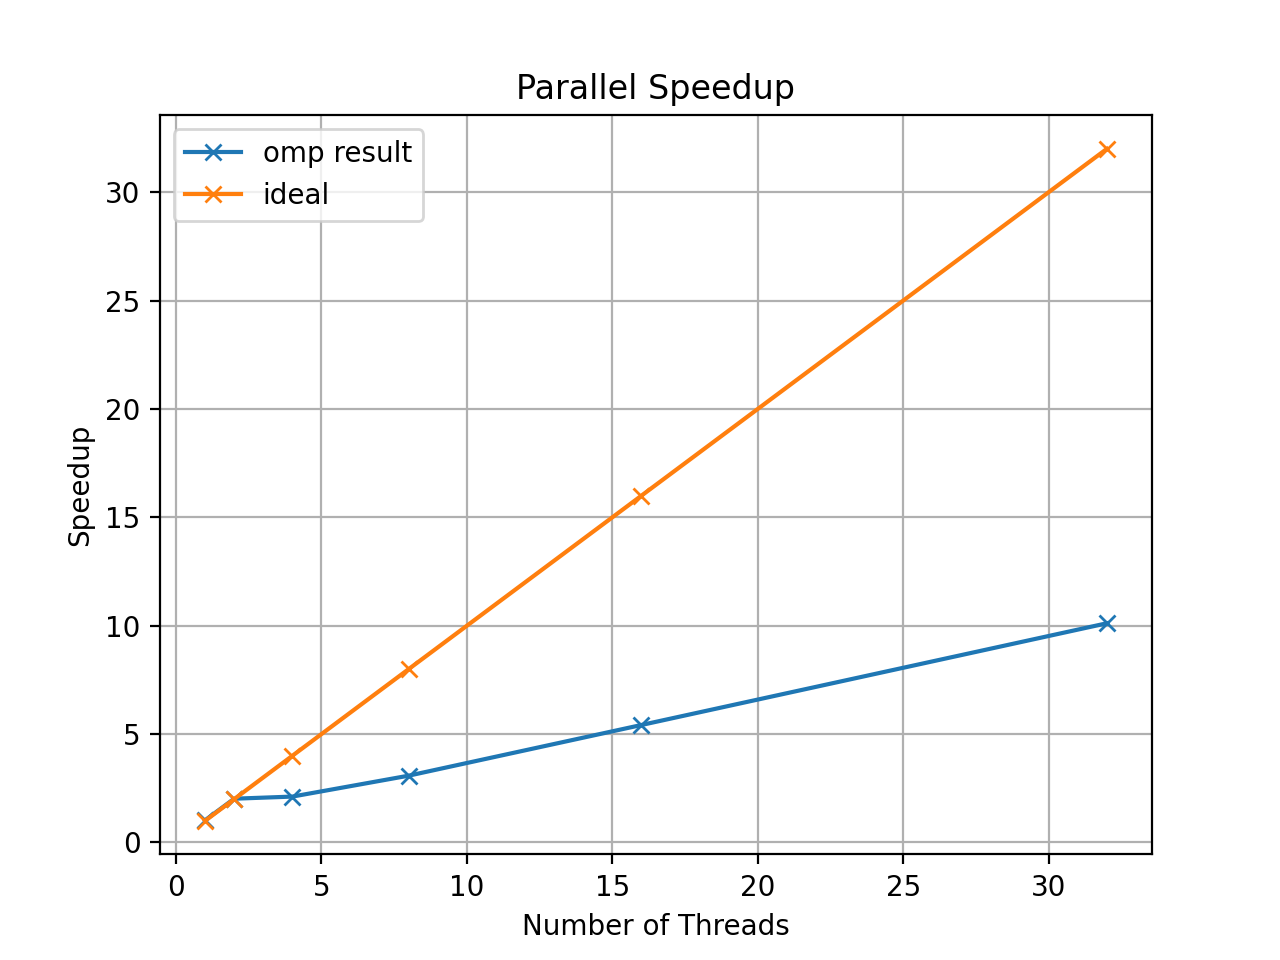
\includegraphics[width=0.8\textwidth]{Images_Output/mandel_speedup.png}
  \caption{Strong Scaling Analysis of the Mandelbrot Set Simulation}
  \label{fig:s_mandel}
\end{figure}

\section{Bug hunt [10 points]}
\subsection{Bug 1}
\indent
The problem here is the combination of \#pragma omp parallel and \#pragma omp for, which leads to an error in this implementation.
Also another problem is that the \#pragma omp for should be followed directly with a for loop and no code in between. Thus, this 
problem can be resolved by first defining the omp parallel region followed by the omp for pragma as illustrated in figure \ref{fig:bug_1}.
\begin{figure}[H]
  \centering
  {\fontsize{8}{10}\selectfont
  \VerbatimInput{Images_Output/bug_1.txt}}
  \caption{Bug 1 resolved}
  \label{fig:bug_1}
\end{figure}

\subsection{Bug 2}
\indent
One major problem here is the fact that further specifications of private and shared variables is missing. Since the pragma omp for is 
used the variable total is unique for each thread and as a result we would run into a racing problem. This can be avoided by introducing 
a total variable that is private for each thread and in the end define a critical region or use the atomic pragma for the global total 
variable. Furthermore, every variable declared outside of the omp region is by default shared. Since, we need to update total in the end, 
this variable needs to be shared. This is not true though for the variable tid, which needs to private and not shared, since each thread 
should hold its own tid value. Otherwise there would be problems with the if condition. In addition, another way instead of defining a 
critical region would be to work with the reduction method presented in Chapter 1.

\subsection{Bug 3}
\indent
the pragma omp sections allows us to define one or more specific sections where only one thread executes the region. Thus the pragma omp barrier 
in line 79 of the provided file \texttt{omp\_bug3.c} will lead to a stop of the whole program, since not more than one thread are already in one region 
and the function print\_results is only called within a section. As a result by only deleting this one line, the code should work as intended.

\subsection{Bug 4}
\indent
Since given the hint from stackoverflow we can identify that the underlying problem here is a segmentation fault. One way to avoid this problem 
is by controlling the stack size limit. The issue here is that the variable a is huge and it's a private variable. Thus, each thread holds a copy 
of the variable a, which leads to the described problem. One way to easily resolve this issue is by granting each thread the possibility of allocating 
more memory to fit the requirement. This could be done for instance by defining in the bashfile a propriate amount with the command \textit{export OMP\_STACKSIZE}. 
For this specific case at least 8.8MB of memory are required, since the problem size N is equal to 1048. Moreover, due to the fact that 1 double requires 8 Bytes, 
the total amount of memory necessary would be 1048 $\cdot$ 1048 $\cdot$ 8 Bytes = 8.786432 MB. 

\subsection{Bug 5}
\indent
The last bug is the issue of a so called deadlock occuring. As already explained an omp section can only by entered by one single thread. 
Hence, in the first section this single thread first sets locka and then lockb, where in the second section another single thread sets concurrently 
lockb and then locka. As a result, both threads are waiting for the other one to unset the underlying lock and the code runs infinatelly long. 
This problem can easily be avoided by rearranging the locks that each thread is able to lock and unlock the given section. More precisely, 
declaring the array both threads need to lock and unlock this process concurrently. Same thing needs to happen for the second part of the code 
where the declaration of the other array follows concurrently.

\section{Parallel histogram calculation using \texttt{OpenMP} [15 points]}
\indent
The idea, how to parallelize the problem on the right hand side of the figure \ref{fig:hist_code}, is represented 
on the left hand side of the same image. The idea is to allocate n number of threads and for each thread a distribution 
variable (dist\_local) should be created, where each thread should iterate over a truncated series of the total vector ($\#$pragma omp for). 
As a result, in the end I still need to avoid racing when updating the target variable (dist). This can be done by making use 
of the pragma omp atomic. An advantage of this pragma is that it allows not only the control of concurrent threads, but also 
grants read and access rights to only a specific memory location, thus sharing similarities with the critical pragma. To make the code on 
the left hand side of image \ref{fig:hist_code} even more efficient, it would be possible to use a reduction clause for the variable dist.
\begin{figure}[H]
  \centering
  {\fontsize{8}{10}\selectfont
  \VerbatimInput{Images_Output/hist_code.txt}}
  \caption{Parallelization of the Histogram Calculation}
  \label{fig:hist_code}
\end{figure}
\indent
Again a strong scaling analysis was conducted and the result can be observed in figure \ref{fig:hist_speedup}. From this plot it 
becomes evident that the speedup approaches a stationary value around 10. Initally the speedup is again close to the ideal value but then 
becomes worse over an increasing number of threads. One reason also here is the increasing overhead to reach the goal with an increasing 
amount of threads. The teamsize, as well as the two operations forking and joining becomes more effort and requires more time. Since our 
problem size stays the same this can lead to an increased overhead and makes the overall code even less efficient in some cases (see previous 
examples). Furthermore, a small snapshot of the results can be found in figure \ref{fig:output_hist}, while the complete output file is 
available in the respective coding directory.
\begin{figure}[H]
  \centering
  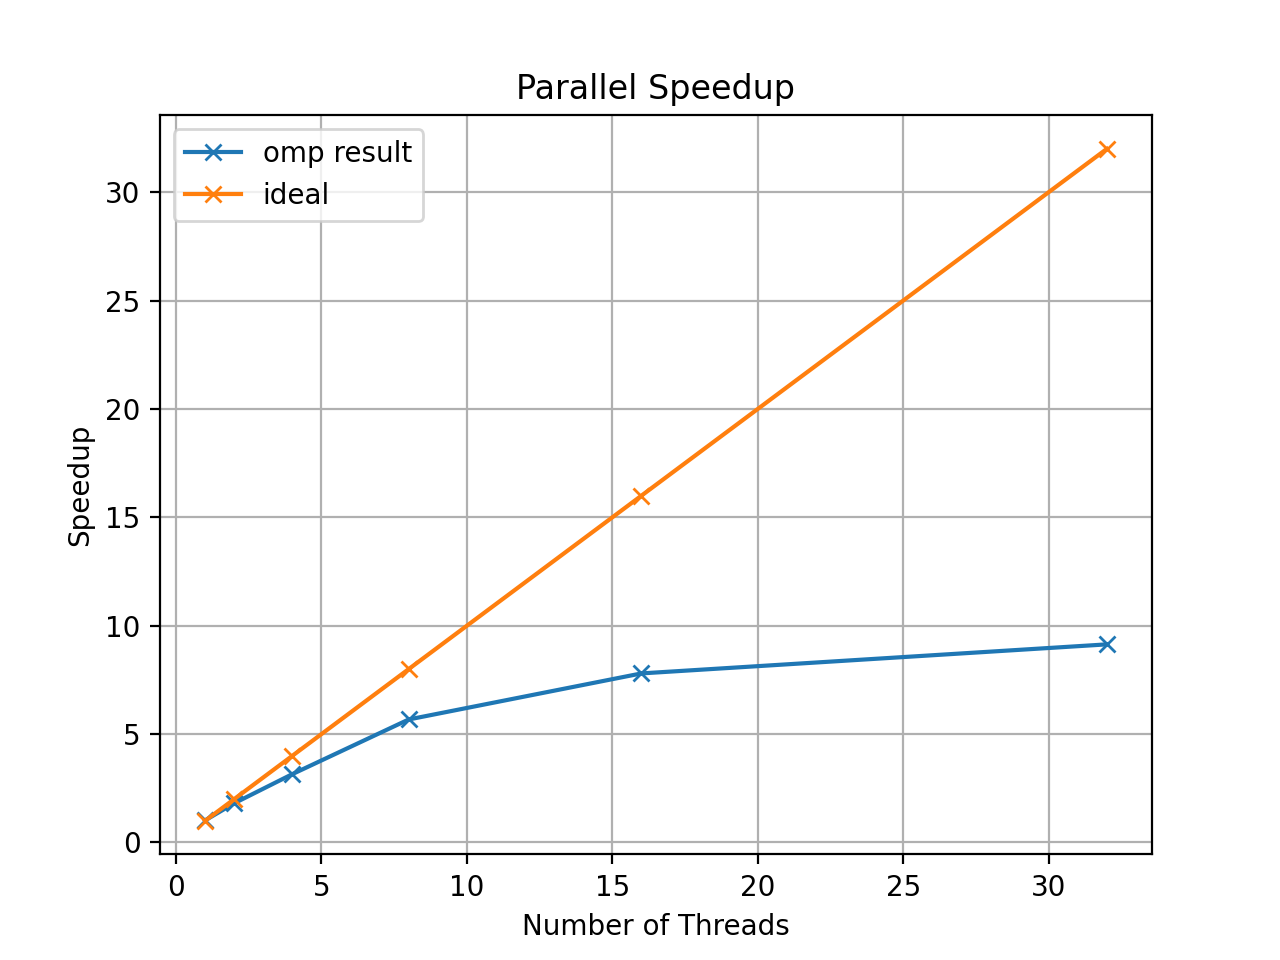
\includegraphics[width=\textwidth]{Images_Output/hist_speedup.png}
  \caption{Strong Scaling Analysis for the Parallel Histogram Calculation}
  \label{fig:hist_speedup}
\end{figure}

\section{Parallel loop dependencies with \texttt{OpenMP} [15 points]}
\indent
This problem was actually introduced in the book \cite{HPC}, as a problem 
which first appeared on the official OpenMP mailing in list in 2007. The 
difficulty in this task is the fact that there is a loop-carried dependency.
Each iteration result depends on the previous one, which makes this task especially 
challenging. Since we truncate/particion the task, it becomes evident that 
a more general formulation is necessary. Thus, the problem can be rewritten as: 
opt[n] = pow(up, n). The problem of this code is that it's computationally expensive 
and we want to avoid it. But still at the first time the code starts and each thread 
runs the task the first time, we want that this computationally more expensive part 
should be used. From that point on, we continue with the faster an computationally 
less expensive algorithm.
\newline \indent
From image \ref{fig:loop-dep}, it is illustrated to face this problem that two 
important clauses were used. One additional clause to the prama for is, firstprivate(lastn).
This clause assigns the initial value of lastn to its private copies when the parallel 
region starts \cite{HPC}. This copy could also have been done manually, but this is just 
a more efficient and automized way. Next clause is lastprivate(Sn) which ensures that 
Sn has the same value as in the serial case after the loop is finished \cite{HPC}. Since 
no results were expected according to the task description, I still put the output of my 
parallelized results into the Appendix, more precisely, figure \ref{fig:output_l-d}.
\begin{figure}[H]
  \centering
  {\fontsize{8}{10}\selectfont
  \VerbatimInput{Images_Output/loop-dependencies-code.txt}}
  \caption{Parallelized Code Snippet}
  \label{fig:loop-dep}
\end{figure}

\section{Quicksort using \texttt{OpenMP} tasks [20 points]}
\indent
Eventhough figure \ref{fig:parallel_quicksort} is in german, it becomes clear how this code 
can be parallelized. The quicksort algorithm seperates the code at each step into a left 
and right branch, we can use this fact to parallelize each division and increase the number 
of threads while going down the tree. Since this problem can be described in form of a binary 
tree structure.
\newline \indent
The underlying code can be found in the respective repository and is named as \texttt{quicksort\_omp.c}. All 
the data and also the length of the container that needs to be sorted, needs to be shared hence they are declared as 
such. First used pragma is omp single which identifies a section of the code that must be run by a single available thread.
Moreover, the additional clause nowait, is used to avoid a barrier at the end of the single directive. One 
approach to solve this problem and the idea described above, is to use omp sections. Since I struggled and got bad 
results with that appraoch I used the omp task pragma instead. This pragma can be used to explicitly define a 
task. According to the IBM website this code gets used a lot to parallelize irregular algorithms. Which is definatelly 
the case for this binary tree. Since it is typically unbalanced as well instead of following a balanced tree structure. 
Again the additional clause firstprivate was used to create copies. For more information return to Chapter 5.
\newline \indent
The resulting figure \ref{fig:quicksort} shows that overhead doesn't get less with an increased problem size. It becomes 
evident that the following parallelized code performs poorly for an increasing number of threads and is far away from the 
theoretical ideal result. The complete output results can be found in the respective repository but for a fixed problem size the 
results can also be found in the Appendix within figure \ref{fig:output_quicksort}.
\begin{figure}[H]
  \centering
  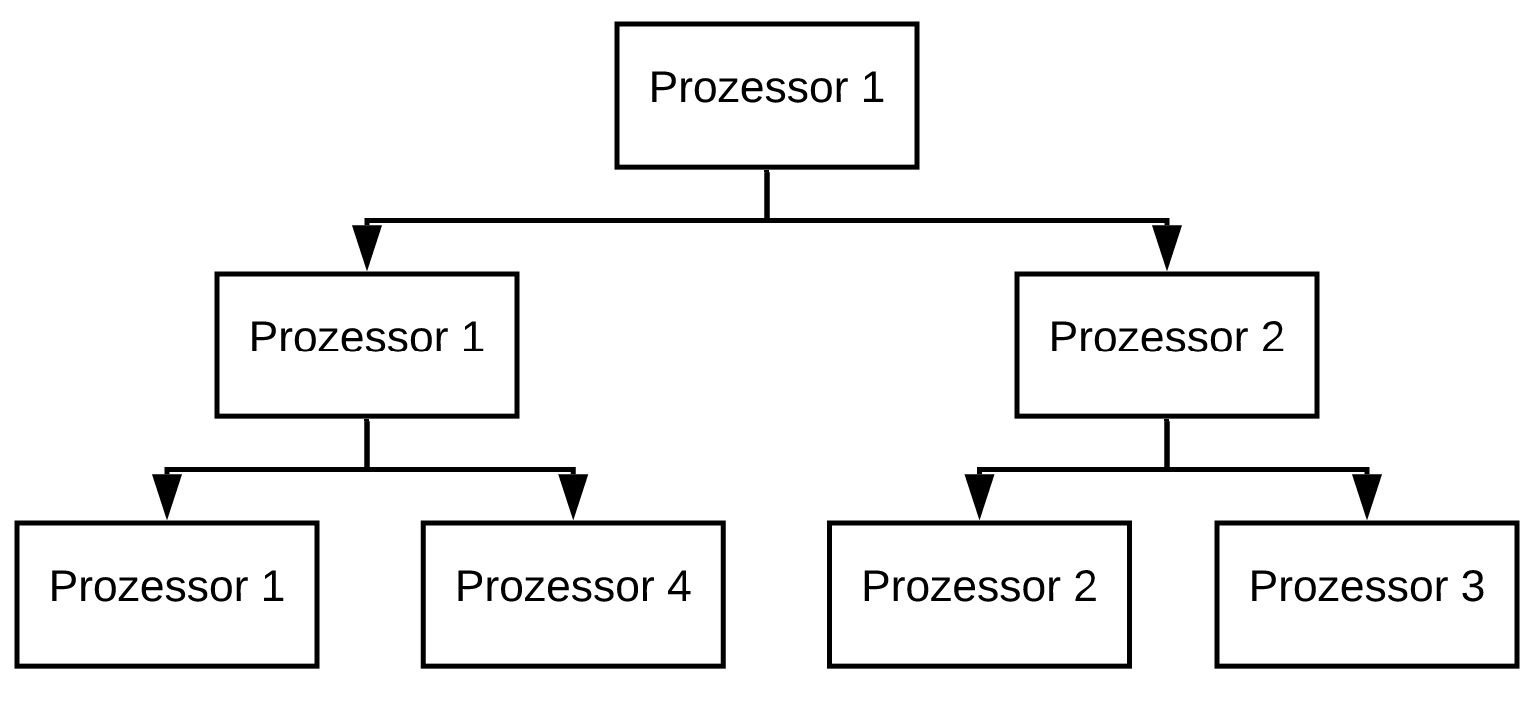
\includegraphics[width=\textwidth]{Images_Output/Parallel_Quicksort.png}
  \caption{Parallelized quicksort algorithm, retrived from \cite{parallelized_quicksort}}
  \label{fig:parallel_quicksort}
\end{figure}

\begin{figure}[H]
  \centering
  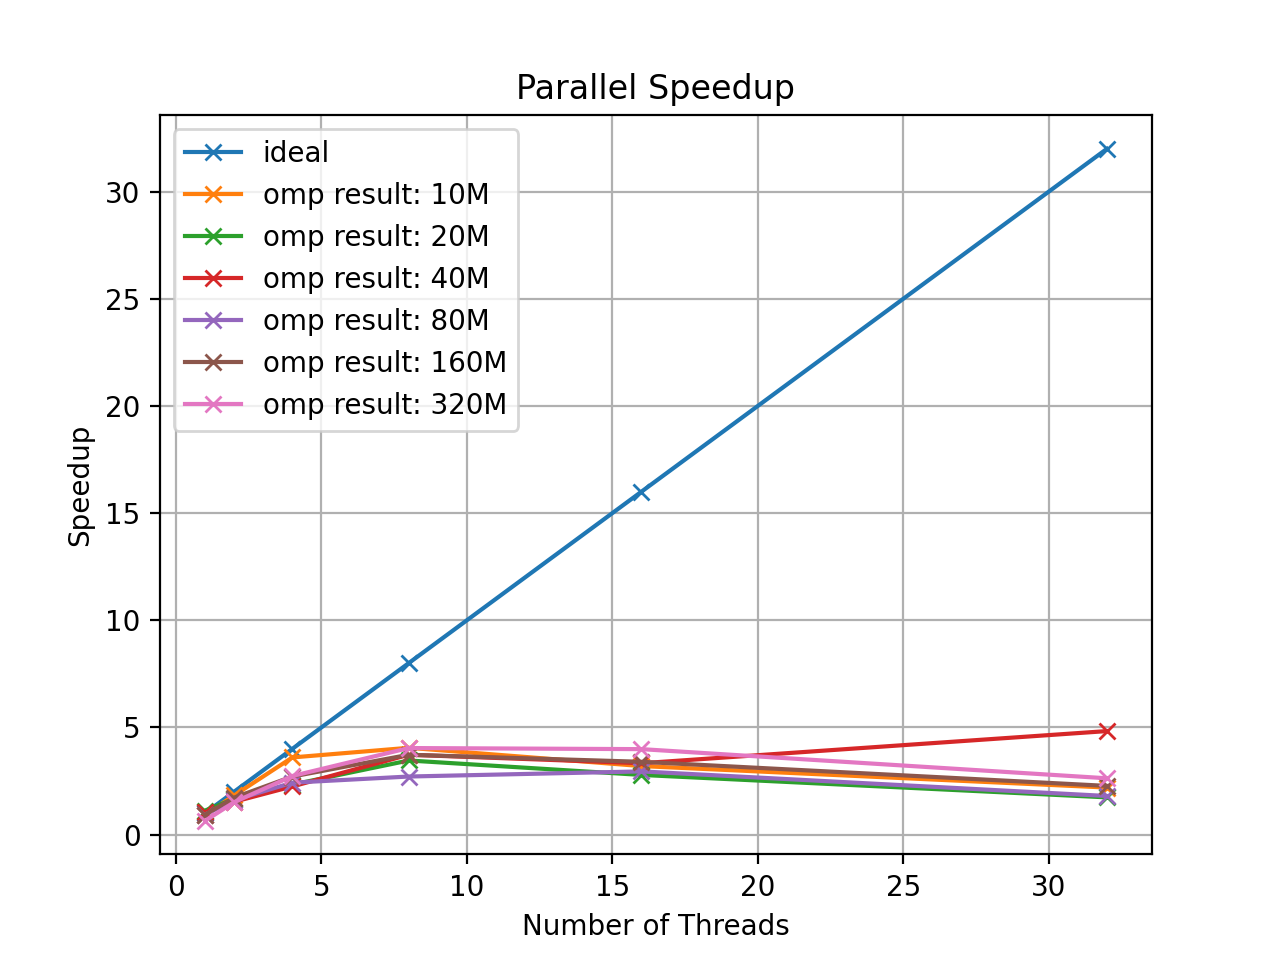
\includegraphics[width=\textwidth]{Images_Output/qicksort_tot_plot.png}
  \caption{Result of the Parallelized Quicksort Algorithm for different Problem Sizes}
  \label{fig:quicksort}
\end{figure}

\newpage
\section{Appendix}% Add to table of contents without numbering
In this section all results and the complete output data can be found.
\begin{figure}[H]
  \centering
  {\fontsize{8}{10}\selectfont
  \VerbatimInput{Images_Output/output_quicksort.txt}}
  \caption{Output File for the Quicksort Problem}
  \label{fig:output_quicksort}
\end{figure}

\begin{figure}[H]
  \centering
  {\fontsize{8}{10}\selectfont
  \VerbatimInput{Images_Output/hist_output.txt}}
  \caption{Output File for the Histogram Calculation Problem}
  \label{fig:output_hist}
\end{figure}

\begin{figure}[H]
  \centering
  {\fontsize{8}{10}\selectfont
  \VerbatimInput{Images_Output/output_mandel.txt}}
  \caption{Output File for the Mandelbrot Set Problem}
  \label{fig:output_mandel}
\end{figure}

\begin{figure}[H]
  \centering
  {\fontsize{8}{10}\selectfont
  \VerbatimInput{Images_Output/output_recur.txt}}
  \caption{Output File for the Loop-Dependencies Problem}
  \label{fig:output_l-d}
\end{figure}

\newpage
% \section*{References}  % Use \section* to prevent section number
\addcontentsline{toc}{section}{References}  % Add to table of contents without numbering

\bibliographystyle{unsrt}
\bibliography{library}


\end{document}
